% Options for packages loaded elsewhere
\PassOptionsToPackage{unicode}{hyperref}
\PassOptionsToPackage{hyphens}{url}
\PassOptionsToPackage{dvipsnames,svgnames,x11names}{xcolor}
%
\documentclass[
  11pt,
]{article}
\usepackage{amsmath,amssymb}
\usepackage{iftex}
\ifPDFTeX
  \usepackage[T1]{fontenc}
  \usepackage[utf8]{inputenc}
  \usepackage{textcomp} % provide euro and other symbols
\else % if luatex or xetex
  \usepackage{unicode-math} % this also loads fontspec
  \defaultfontfeatures{Scale=MatchLowercase}
  \defaultfontfeatures[\rmfamily]{Ligatures=TeX,Scale=1}
\fi
\usepackage[]{mathptmx}
\ifPDFTeX\else
  % xetex/luatex font selection
\fi
% Use upquote if available, for straight quotes in verbatim environments
\IfFileExists{upquote.sty}{\usepackage{upquote}}{}
\IfFileExists{microtype.sty}{% use microtype if available
  \usepackage[]{microtype}
  \UseMicrotypeSet[protrusion]{basicmath} % disable protrusion for tt fonts
}{}
\makeatletter
\@ifundefined{KOMAClassName}{% if non-KOMA class
  \IfFileExists{parskip.sty}{%
    \usepackage{parskip}
  }{% else
    \setlength{\parindent}{0pt}
    \setlength{\parskip}{6pt plus 2pt minus 1pt}}
}{% if KOMA class
  \KOMAoptions{parskip=half}}
\makeatother
\usepackage{xcolor}
\usepackage[margin=1in]{geometry}
\usepackage{longtable,booktabs,array}
\usepackage{calc} % for calculating minipage widths
% Correct order of tables after \paragraph or \subparagraph
\usepackage{etoolbox}
\makeatletter
\patchcmd\longtable{\par}{\if@noskipsec\mbox{}\fi\par}{}{}
\makeatother
% Allow footnotes in longtable head/foot
\IfFileExists{footnotehyper.sty}{\usepackage{footnotehyper}}{\usepackage{footnote}}
\makesavenoteenv{longtable}
\usepackage{graphicx}
\makeatletter
\def\maxwidth{\ifdim\Gin@nat@width>\linewidth\linewidth\else\Gin@nat@width\fi}
\def\maxheight{\ifdim\Gin@nat@height>\textheight\textheight\else\Gin@nat@height\fi}
\makeatother
% Scale images if necessary, so that they will not overflow the page
% margins by default, and it is still possible to overwrite the defaults
% using explicit options in \includegraphics[width, height, ...]{}
\setkeys{Gin}{width=\maxwidth,height=\maxheight,keepaspectratio}
% Set default figure placement to htbp
\makeatletter
\def\fps@figure{htbp}
\makeatother
\setlength{\emergencystretch}{3em} % prevent overfull lines
\providecommand{\tightlist}{%
  \setlength{\itemsep}{0pt}\setlength{\parskip}{0pt}}
\setcounter{secnumdepth}{5}
\usepackage{caption}
\captionsetup{labelformat=empty,font=small,justification=raggedright,singlelinecheck=false}
\DeclareUnicodeCharacter{2212}{\ensuremath{-}}
\usepackage{etoolbox}
\AtBeginEnvironment{longtable}{\small}
\setlength{\emergencystretch}{3em}
% natbib redefines \bibsection when it is loaded (after this header); the manuscript has its own "References" heading, so drop the second one
\AtBeginDocument{\renewcommand{\bibsection}{}}
\ifLuaTeX
  \usepackage{selnolig}  % disable illegal ligatures
\fi
\usepackage[round]{natbib}
\bibliographystyle{plainnat}
\IfFileExists{bookmark.sty}{\usepackage{bookmark}}{\usepackage{hyperref}}
\IfFileExists{xurl.sty}{\usepackage{xurl}}{} % add URL line breaks if available
\urlstyle{same}
\hypersetup{
  pdftitle={Query-Variation Robustness of Sparse, Latent-Semantic and Fused First-Stage Retrieval: A Reproducible Pilot Study on the Vaswani Collection},
  pdfauthor={{[}HUMAN AUTHOR(S) TO COMPLETE{]}},
  colorlinks=true,
  linkcolor={Maroon},
  filecolor={Maroon},
  citecolor={Blue},
  urlcolor={Blue},
  pdfcreator={LaTeX via pandoc}}

\title{Query-Variation Robustness of Sparse, Latent-Semantic and Fused
First-Stage Retrieval: A Reproducible Pilot Study on the Vaswani
Collection}
\author{{[}HUMAN AUTHOR(S) TO COMPLETE{]}}
\date{Draft of October 2026}

\begin{document}
\maketitle
\begin{abstract}
Query-variation robustness asks whether a retrieval system keeps working
when the same information need is worded differently. This paper reports
a small pilot on the Vaswani/NPL collection (11,429 abstracts, 93
queries), with the analysis plan written before the run. It compares
three first-stage systems: BM25, a non-neural latent-semantic-analysis
(LSA) retriever, and their reciprocal-rank-fusion (RRF) hybrid. Using
the four meaning-preserving categories of Penha et al., 644 query
rewrites were kept for analysis. Misspellings changed nDCG@10 by −18.5\%
(BM25), −21.4\% (LSA) and −20.2\% (hybrid); all three Holm-adjusted
p-values are below 0.001. Paraphrasing changed BM25 by −13.3\% (Holm p =
0.004), whereas the changes for LSA (−5.3\%) and the hybrid (−7.8\%)
were not significant after correction. Natural-question rewrites and
stop-word removal moved nDCG@10 by less than 2\% for every system, and
word-order changes had exactly zero effect, as they must for
bag-of-words systems. Paraphrasing changed the top ten results more than
misspelling did but cost less effectiveness, so ranking stability did
not track harm across categories. Within each system it did track harm
across individual rewrites (Spearman correlation −0.60 to −0.67). The
pilot has hard limits. It uses one small, old collection and no neural
retriever. No rewrite was checked by a human: typos are assumed to keep
their meaning because of how they are made, and the other rewrites were
reviewed by a single LLM from the generator's model family. The
literature search was not systematic. Code, rewrites, rankings and 85
automated tests are released.

\textbf{Keywords:} information retrieval; query variation; retrieval
robustness; BM25; latent semantic analysis; rank fusion; reproducibility
\end{abstract}

\begin{quote}
\textbf{Status of this draft.} Pilot study. The code, the rewrites, the
experiments and this text were produced by an AI system (Section 8). No
human has yet read, verified or approved it. Neural dense retrievers,
BEIR datasets and human validation of the query rewrites are \emph{not}
part of it. Text in square brackets is for the human author to complete;
only people who made a substantial scholarly contribution, have read and
verified this work, and accept responsibility for it may be listed as
authors.
\end{quote}

\hypertarget{introduction}{%
\section{Introduction}\label{introduction}}

A retrieval benchmark fixes one wording of each information need, but
users word the same need in many ways. Whether a system's score survives
a change of wording is a different question from how high the score is.
Query variability has a long research history: the UQV100 test
collection was created to study it \citep{bailey2016}; later work
examines retrieval consistency in the presence of query variations
\citep{bailey2017} and evaluation pooled over query variations
\citep{moffat2015}; and a line of work shows that neural rankers and
retrievers lose effectiveness when queries contain typos
\citep{zhuang2021, zhuang2022, sidiropoulos2022, tasawong2023}.
\citet{penha2022} organise query variations into a taxonomy, provide
generators for them and show that retrieval pipelines lose a substantial
share of their effectiveness under syntax-changing variations;
\citet{hagen2024} reproduce that study and extend it to newer neural
models.

This paper does not claim that query-variation robustness is a new
problem. It is a small pilot with a narrower aim: to build and check a
transparent pipeline, and to measure on one collection how three
first-stage systems respond to rewording. The systems are BM25, a
non-neural latent-semantic retriever and their reciprocal-rank-fusion
hybrid \citep{cormack2009}. The rewrites come from the four
meaning-preserving categories of \citet{penha2022}, and for each system
the study looks at effectiveness and at how much the top-ranked results
move. The statistics are paired and clustered by query, and every
analysis step was fixed in writing before the run.

Two research questions are addressed. \textbf{RQ1:} how does
effectiveness change under each variation category? \textbf{RQ2:} do the
three systems respond differently? Two further questions from the
original research plan, whether effects vary across domains (RQ3) and
whether degradation can be predicted on held-out domains (RQ4), are out
of scope because the pilot has one collection.

The work was done in a sandbox that could install software packages but
could not download neural model weights or BEIR datasets
\citep{thakur2021}. Everything that could be run was run. The code for
the rest was written and tested with a stand-in encoder but has never
been run on real data. Nothing in this paper is a result about neural
dense retrievers or about other domains.

The contributions are modest and are stated as such:

\begin{enumerate}
\def\labelenumi{\arabic{enumi}.}
\tightlist
\item
  An open, tested pipeline (BM25, LSA, RRF, five effectiveness and
  stability measures, cluster bootstrap, permutation tests with Holm
  correction) with an account of the defects found in the starter code
  this work began from (Section 3.7).
\item
  Effect sizes with intervals for the four categories and three systems
  on one collection (Section 4), computed from a plan written before the
  run (Section 3.6).
\item
  Three observations that are worth testing at scale rather than
  believing from this pilot: ranking stability and effectiveness loss
  are not interchangeable across categories; the ``paraphrasing''
  category hides a large difference between generators; and a hybrid of
  two whole-word systems lies between its components rather than beating
  both (Sections 4.3 to 4.5).
\item
  A clear account of what the validity of the rewrites does and does not
  rest on (Section 3.3), because that validity is the weakest link in
  this kind of study.
\end{enumerate}

\hypertarget{related-work}{%
\section{Related work}\label{related-work}}

\hypertarget{query-variability-and-ranking-consistency}{%
\subsection{Query variability and ranking
consistency}\label{query-variability-and-ranking-consistency}}

UQV100 is a test collection created to study query variability
\citep{bailey2016}. \citet{bailey2017} study retrieval consistency in
the presence of query variations, and \citet{moffat2015} study
evaluation pooled over query variations. More recently,
\citet{alaofi2023} explored whether generative language models can
create query variants for test collections, and \citet{campese2025}
propose a training loss that penalises differences between the documents
retrieved for semantically equivalent queries (read at abstract level
only). This line of work establishes that wording sensitivity and
ranking consistency are old topics; the contribution of the present
pilot cannot be the question itself.

\hypertarget{robustness-of-neural-retrievers-and-typos}{%
\subsection{Robustness of neural retrievers and
typos}\label{robustness-of-neural-retrievers-and-typos}}

A group of papers examines typos in neural retrieval and proposes
training remedies: BERT-based passage retrieval and ranking
\citep{zhuang2021}, dense retrievers with CharacterBERT and
self-teaching \citep{zhuang2022}, an analysis of dual encoders against
misspellings \citep{sidiropoulos2022}, typo-robust representation
learning \citep{tasawong2023} and multi-positive contrastive learning
\citep{sidiropoulos2024}. \citet{penha2022} define a taxonomy of query
variations with generators and evaluate BM25 followed by neural
re-rankers on two collections, reporting a loss of roughly one fifth of
effectiveness on average under their variations (read through a page
summariser; see Appendix A). \citet{hagen2024} reproduce that study for
BERT- and T5-based re-rankers and extend it to Sentence-BERT,
CharacterBERT-based, E5-Mistral, AnglE and Ada v2 models; from the parts
read, they evaluate the re-ranking stage rather than the whole pipeline.
\citet{li2026} study LLM-based dense retrievers and report that they are
more robust to typos than encoder-only baselines but remain vulnerable
to semantic perturbations such as synonym substitution (abstract only),
and \citet{percin2025} report that retrievers in retrieval-augmented
generation degrade under minor query variations (abstract only).

\hypertarget{fusion-and-the-gap-this-pilot-does-and-does-not-address}{%
\subsection{Fusion, and the gap this pilot does and does not
address}\label{fusion-and-the-gap-this-pilot-does-and-does-not-address}}

Reciprocal rank fusion combines rankings by summing reciprocal ranks and
is a simple, nearly parameter-free way to merge a lexical and a semantic
ranking \citep{cormack2009}. Whether a fused first stage inherits,
averages or compounds the sensitivities of its components under query
variation is an empirical question. In the sources read for this study
(Appendix A), robustness is measured for re-rankers placed on top of
BM25 \citep{penha2022, hagen2024} or for single dense or LLM-based
retrievers \citep{li2026, percin2025}, and none of them, as far as could
be seen from the parts read, reports a fused lexical-semantic first
stage next to its own components under the \citet{penha2022} categories
with paired, query-clustered inference.

This observation is weak evidence of a gap, not a demonstration. The
literature search was not systematic (Appendix A), several sources were
read only at abstract level, and the 2025 and 2026 literature is large.
The pilot does not close the gap either: its ``semantic'' component is
non-neural LSA, so it cannot test whether a neural retriever and BM25
complement each other under query variation. The most that can be
claimed is a transparent, reproducible starting point.

\hypertarget{experimental-design}{%
\section{Experimental design}\label{experimental-design}}

\hypertarget{collection}{%
\subsection{Collection}\label{collection}}

The Vaswani (NPL) collection has 11,429 abstracts of physics and
electronics literature, 93 queries and 2,083 relevance judgments, all
binary; every query has at least one relevant document and no judged
document is missing from the corpus. The counts agree with the
description on the ir\_datasets page \citep{irdatasets_vaswani}. The
collection is small and old, and neither that page nor the Glasgow IR
group page for the collection \citep{glasgow_npl} states its provenance
details or a licence; the latter also carries a caution about the
collection. For that reason the collection is not redistributed:
\texttt{scripts/fetch\_vaswani.py} downloads it from a pinned commit of
the PyTerrier repository and verifies SHA-256 and md5 checksums (the md5
values equal those PyTerrier itself lists for its Vaswani resources; no
checksum from the collection's original authors was found). Whoever runs
the script is responsible for checking the terms of use.

\hypertarget{systems}{%
\subsection{Systems}\label{systems}}

All systems return their top 100 documents and share one analyzer:
lowercasing, \texttt{{[}a-z0-9{]}+} tokens, the 33-word Lucene English
stop list and Porter stemming \citep{porter1980}.

\begin{itemize}
\tightlist
\item
  \textbf{BM25} \citep{robertson2009}: an own sparse-matrix
  implementation with Lucene-style IDF, \(k_1 = 1.20\) and \(b = 0.75\)
  (common default values; not tuned on any query), query-term
  multiplicity counted, documents with score zero not returned. Its
  scores were checked against the \texttt{bm25s} package.
\item
  \textbf{LSA}: TF-IDF with sublinear term frequency on the same
  analyzer, truncated SVD to 300 dimensions (random seed 0)
  \citep{deerwester1990}, L2 normalisation and exact cosine search. LSA
  is a latent-semantic retriever, \textbf{not a neural one}. It stands
  in for the ``dense'' component of the original plan and is not
  evidence about neural dense retrievers. Like BM25 it works on whole
  words of the collection's vocabulary.
\item
  \textbf{RRF hybrid}: reciprocal rank fusion with \(k = 60\) over the
  two top-100 lists \citep{cormack2009}.
\end{itemize}

A sentence-embedding retriever and its hybrid are implemented and
unit-tested with a stand-in encoder but were not run, because no model
weights were available.

\hypertarget{query-variations-and-their-validity}{%
\subsection{Query variations and their
validity}\label{query-variations-and-their-validity}}

Categories follow the four meaning-preserving classes of
\citet{penha2022}: misspelling, ordering, naturality and paraphrasing.
The two meaning-changing classes (generalisation and specialisation,
aspect change) are not studied. Generator names follow theirs where they
exist; the code is an independent re-implementation. Table 1 lists the
generators and what happened to their 734 candidate rewrites.

\begin{longtable}[]{@{}
  >{\raggedright\arraybackslash}p{(\columnwidth - 10\tabcolsep) * \real{0.1263}}
  >{\raggedright\arraybackslash}p{(\columnwidth - 10\tabcolsep) * \real{0.2632}}
  >{\raggedright\arraybackslash}p{(\columnwidth - 10\tabcolsep) * \real{0.1368}}
  >{\raggedleft\arraybackslash}p{(\columnwidth - 10\tabcolsep) * \real{0.1158}}
  >{\raggedleft\arraybackslash}p{(\columnwidth - 10\tabcolsep) * \real{0.0737}}
  >{\raggedright\arraybackslash}p{(\columnwidth - 10\tabcolsep) * \real{0.2842}}@{}}
\caption{Table 1. Query rewrites by generator. \emph{Candidates} are all
rewrites produced; \emph{kept} are those used in the analysis. No
rewrite is human-verified (Section 3.3).}\tabularnewline
\toprule\noalign{}
\begin{minipage}[b]{\linewidth}\raggedright
Category
\end{minipage} & \begin{minipage}[b]{\linewidth}\raggedright
Generator
\end{minipage} & \begin{minipage}[b]{\linewidth}\raggedright
Produced by
\end{minipage} & \begin{minipage}[b]{\linewidth}\raggedleft
Candidates
\end{minipage} & \begin{minipage}[b]{\linewidth}\raggedleft
Kept
\end{minipage} & \begin{minipage}[b]{\linewidth}\raggedright
Basis of validity
\end{minipage} \\
\midrule\noalign{}
\endfirsthead
\toprule\noalign{}
\begin{minipage}[b]{\linewidth}\raggedright
Category
\end{minipage} & \begin{minipage}[b]{\linewidth}\raggedright
Generator
\end{minipage} & \begin{minipage}[b]{\linewidth}\raggedright
Produced by
\end{minipage} & \begin{minipage}[b]{\linewidth}\raggedleft
Candidates
\end{minipage} & \begin{minipage}[b]{\linewidth}\raggedleft
Kept
\end{minipage} & \begin{minipage}[b]{\linewidth}\raggedright
Basis of validity
\end{minipage} \\
\midrule\noalign{}
\endhead
\bottomrule\noalign{}
\endlastfoot
misspelling & \texttt{NeighbCharSwap} & seeded code & 93 & 93 & by
construction \\
misspelling & \texttt{RandomCharSub} & seeded code & 93 & 93 & by
construction \\
misspelling & \texttt{QWERTYCharSub} & seeded code & 93 & 93 & by
construction \\
paraphrasing & \texttt{LLM\_Paraphrase} & AI assistant & 93 & 93 & LLM
review \\
paraphrasing & \texttt{LLM\_SynonymSwap} & AI assistant & 93 & 92 & LLM
review \\
naturality & \texttt{LLM\_NaturalQuestion} & AI assistant & 93 & 92 &
LLM review \\
naturality & \texttt{RemoveStopWords} & code & 83 & 80 & LLM review +
assistant recheck \\
ordering & \texttt{RandomOrderSwap} & seeded code & 93 & 8 & LLM review
+ function-word rule \\
\textbf{all} & & & \textbf{734} & \textbf{644} & \\
\end{longtable}

\emph{Misspellings} are seeded character edits of one word of at least
four letters (adjacent swap, random substitution, substitution by a
neighbouring key on a QWERTY keyboard). They are treated as
meaning-preserving by construction. That is an assumption: an edit that
happens to create another real word could change the meaning. Section
4.7 counts how often that happened with respect to the collection's
vocabulary (0 of 279). \emph{Word-order swaps} exchange two words with
different surface forms, and \emph{stop-word removal} deletes every word
of the NLTK English stop-word list. Both are machine-made (455
machine-made candidates in all, including the typos).

The remaining 279 rewrites (a natural-language question, a differently
structured paraphrase and a synonym swap for each query) were written by
hand in three batches by the AI assistant that also wrote the code.
There was no separate prompt, sampling setting or seed to record, so the
rewrites are stored verbatim. The assistant saw the queries and the
collection's vocabulary but no retrieval output.

\emph{Validity of the non-typo rewrites.} A reviewer saw only the
(original, rewrite) pairs, in shuffled order with opaque identifiers and
without category or generator, and labelled each pair
\texttt{equivalent}, \texttt{broader}, \texttt{narrower} or
\texttt{different}. The reviewer was three sequential agents run with a
smaller Claude model setting. Generator and reviewer belong to the same
model family, so shared blind spots are possible. The reviewer prompt is
reproduced verbatim in the repository. Thirty typo rewrites were mixed
into the packets as a calibration sample, and the reviewer labelled all
of them \texttt{equivalent}; that result is a diagnostic only and never
changed the status of a typo.

The reviewer accepted 47 of the 93 word-order swaps, including garbled
ones, which the assistant judged too lenient. Before any retrieval
output on the pilot queries had been seen, a stricter second rule was
therefore added (amendment A4): a swap is accepted only if every word
that moved is a function word, and a rewrite of the swap or stop-word
kind enters the analysis only if reviewer and rule agree. The same
assistant that wrote the code and the rewrites made the rule and the
recheck, so they are stricter but not independent. Of the 734
candidates, 644 were kept (279 by construction and 365 after LLM
review); 90 were dropped, 85 of them word-order swaps.

\textbf{No rewrite in this pilot is human-verified.} The analysis is
therefore conditional on the rewrites being meaning-preserving, which
has been checked only by construction and by one LLM reviewer. A blind
sheet of 200 rewrites for a human audit and a tool that scores it are
part of the repository, but the audit has not been done.

\hypertarget{measures}{%
\subsection{Measures}\label{measures}}

The primary measure is nDCG@10 (linear gain, logarithmic discount)
\citep{jarvelin2002}. Secondary measures are Recall@100 and MRR@10
(binary relevance), overlap@10 (the share of the top ten shared by the
rankings for the original query and its rewrite) and extrapolated
rank-biased overlap (RBO, \(p = 0.9\), depth 100) \citep{webber2010}
between those two rankings. Queries without a relevant document would be
excluded; there are none.

\hypertarget{estimands-and-inference}{%
\subsection{Estimands and inference}\label{estimands-and-inference}}

For a system and a category, let \(Q_c\) be the original queries that
have at least one kept rewrite in category \(c\). For each such query
the metric of its rewrites is averaged first, so a query counts once per
category however many rewrites it has. The primary estimand is the
relative change, the mean over \(Q_c\) of the rewrite metric divided by
the mean over \(Q_c\) of the original-query metric, minus one. Intervals
are 95\% percentile \textbf{cluster-bootstrap} intervals that resample
original queries (rewrites of one query are never treated as
independent; 10,000 resamples, seed 20261017). Tests are two-sided
sign-flip permutation tests on the per-query differences, which is a
paired randomisation test of the kind compared by \citet{smucker2007};
they are exact when at most 16 differences are non-zero and otherwise
use 200,000 random flips.

Holm's step-down correction \citep{holm1979} is applied over the primary
family, all 12 system-by-category tests of nDCG@10. Every other p-value,
interval and comparison is descriptive. A category whose interval covers
zero is reported as ``no reliable change detected'', never as ``no
effect''.

The comparison of the hybrid with its components (per-query difference
in absolute nDCG@10 change) and the Spearman correlation between RBO and
the size of the nDCG@10 change over (query, rewrite) pairs are
exploratory; the latter has a cluster-bootstrap interval (2,000
resamples).

\hypertarget{pre-specification-amendments-and-deviations}{%
\subsection{Pre-specification, amendments and
deviations}\label{pre-specification-amendments-and-deviations}}

The analysis plan (\texttt{docs/ANALYSIS\_PLAN.md}) was written on 17
October 2026 before any retrieval run on the pilot queries and fixed the
systems, categories, measures, estimands, inference and cross-checks.
Amendments A1 to A3 (18 October) and the validity rule and reviewer
identity (A4 and A5, decided 19 October) preceded the first run on the
pilot queries, which started at 2026-10-20T06:02:38+00:00. A4 and A5
were written into the plan file only after the run, so the first 8,130
bytes of the file are exactly the plan as it stood at the run; they hash
to \texttt{6d31b030288b1c85...}, the value stored in
\texttt{run\_metadata.json}.

The retrieval code had been exercised only on a synthetic collection;
the real collection was loaded before the run only to check its counts
and to compute the typo-vocabulary diagnostic. Four deviations are
recorded in the plan: the executed validity rule is stricter than the
plan's text (D1); what the collection cross-check does and does not
establish (D2); the blind audit sheet that replaces the older one (D3);
and no deviation in systems, measures, estimands, resampling settings,
multiplicity family, seeds or depth (D4).

The plan is an internal document, not an external preregistration. It
carries no outside timestamp, so the order of events rests on the file
hash, the run metadata and, once published, the repository history.

\hypertarget{verification-of-the-software-and-the-numbers}{%
\subsection{Verification of the software and the
numbers}\label{verification-of-the-software-and-the-numbers}}

The package has 85 automated tests. Own nDCG@10, Recall@100 and MRR@10
equal the output of \texttt{pytrec\_eval} \citep{vangysel2018} and
\texttt{ranx} on the same runs (tolerance \(10^{-9}\)); own BM25 scores
equal \texttt{bm25s}; own RBO equals the \texttt{rbo} package and
satisfies the analytic identities; the bootstrap interval for a mean
agrees with the analytical interval on a large sample and the sign-flip
p-value agrees with \texttt{scipy.stats.permutation\_test} on a small
one. A bug-injection check made 23 deliberate one-line breakages in the
metric, BM25, stability, fusion, ranking, statistics, analysis, run and
rewrite-loading code and the tests caught 22; the survivor is an
equivalent mutant (the base of nDCG's logarithm cancels in nDCG/IDCG).

\texttt{scripts/verify\_results.py} recomputes the effectiveness numbers
of this paper from the saved rankings and the judgments with a separate
plain implementation and compares them with the tables: every per-query
and summary number agrees to machine precision, the intervals and
p-values are re-estimated with fresh Monte-Carlo runs under other seeds
and agree within sampling error, and the provenance hashes match. The
Spearman correlations agree only to within \(10^{-4}\), because exact
ties in the nDCG@10 change are split by floating-point noise in the
pipeline's values; resolving the ties by rounding moves the correlations
by less than \(10^{-4}\), which does not affect the two decimals
reported.

Every experimental number in this manuscript is filled in from the
result files by \texttt{scripts/build\_paper.py}, which also asserts
that each data-dependent sentence below still holds.

The starter script this work began from (a BM25-only scaffold on an
Elasticsearch wrapper) was reviewed and not used. It was not run,
because it needs an Elasticsearch server. Reading it and the library it
calls showed 11 defects, among them an aliased results dictionary that
lets later rewrites overwrite the original-query rankings, a stale
ranking being scored when a rewrite retrieves nothing, a key that does
not exist (so MRR@10 would be silently missing) and a re-index of the
whole corpus on every call (\texttt{docs/STARTER\_CODE\_REVIEW.md}). The
first three would have produced plausible but wrong numbers in a
direction that flatters robustness.

\hypertarget{results}{%
\section{Results}\label{results}}

\hypertarget{baselines}{%
\subsection{Baselines}\label{baselines}}

On the original queries (Table 2) BM25 reaches nDCG@10 = 0.432 (95\% CI
0.375 to 0.489), LSA 0.282 (95\% CI 0.232 to 0.334) and the RRF hybrid
0.382 (95\% CI 0.326 to 0.437). The BM25 and hybrid intervals overlap
substantially, so the pilot does not establish which is better on the
original queries (the difference was not tested). LSA has the lowest
nDCG@10; its interval is separated from BM25's but overlaps the
hybrid's. All values rest on 93 queries and the intervals are wide.

\begin{longtable}[]{@{}
  >{\raggedright\arraybackslash}p{(\columnwidth - 6\tabcolsep) * \real{0.1477}}
  >{\raggedleft\arraybackslash}p{(\columnwidth - 6\tabcolsep) * \real{0.2841}}
  >{\raggedleft\arraybackslash}p{(\columnwidth - 6\tabcolsep) * \real{0.2841}}
  >{\raggedleft\arraybackslash}p{(\columnwidth - 6\tabcolsep) * \real{0.2841}}@{}}
\caption{Table 2. Effectiveness on the original queries (93 queries,
Vaswani). Mean and 95\% percentile bootstrap interval over queries
(10,000 resamples).}\tabularnewline
\toprule\noalign{}
\begin{minipage}[b]{\linewidth}\raggedright
System
\end{minipage} & \begin{minipage}[b]{\linewidth}\raggedleft
nDCG@10
\end{minipage} & \begin{minipage}[b]{\linewidth}\raggedleft
Recall@100
\end{minipage} & \begin{minipage}[b]{\linewidth}\raggedleft
MRR@10
\end{minipage} \\
\midrule\noalign{}
\endfirsthead
\toprule\noalign{}
\begin{minipage}[b]{\linewidth}\raggedright
System
\end{minipage} & \begin{minipage}[b]{\linewidth}\raggedleft
nDCG@10
\end{minipage} & \begin{minipage}[b]{\linewidth}\raggedleft
Recall@100
\end{minipage} & \begin{minipage}[b]{\linewidth}\raggedleft
MRR@10
\end{minipage} \\
\midrule\noalign{}
\endhead
\bottomrule\noalign{}
\endlastfoot
BM25 & 0.432 {[}0.375, 0.489{]} & 0.601 {[}0.552, 0.649{]} & 0.685
{[}0.603, 0.763{]} \\
LSA & 0.282 {[}0.232, 0.334{]} & 0.495 {[}0.442, 0.548{]} & 0.506
{[}0.418, 0.593{]} \\
RRF hybrid & 0.382 {[}0.326, 0.437{]} & 0.570 {[}0.519, 0.621{]} & 0.642
{[}0.558, 0.723{]} \\
\end{longtable}

\hypertarget{effect-of-the-variation-categories}{%
\subsection{Effect of the variation
categories}\label{effect-of-the-variation-categories}}

Table 3 and Figure 1 give the primary results.

\begin{longtable}[]{@{}
  >{\raggedright\arraybackslash}p{(\columnwidth - 12\tabcolsep) * \real{0.1413}}
  >{\raggedright\arraybackslash}p{(\columnwidth - 12\tabcolsep) * \real{0.1522}}
  >{\raggedleft\arraybackslash}p{(\columnwidth - 12\tabcolsep) * \real{0.1196}}
  >{\raggedleft\arraybackslash}p{(\columnwidth - 12\tabcolsep) * \real{0.1087}}
  >{\raggedleft\arraybackslash}p{(\columnwidth - 12\tabcolsep) * \real{0.1087}}
  >{\raggedleft\arraybackslash}p{(\columnwidth - 12\tabcolsep) * \real{0.2717}}
  >{\raggedleft\arraybackslash}p{(\columnwidth - 12\tabcolsep) * \real{0.0978}}@{}}
\caption{Table 3. Effect of query-variation categories on nDCG@10
(primary analysis, 12 tests). Original and rewrite columns are means
over the queries that have at least one kept rewrite in the category
(each query counts once per category). Relative change is the ratio of
the two means minus one; the interval is a cluster bootstrap over
original queries. Holm \(p\) comes from a two-sided sign-flip
permutation test, adjusted over the 12 tests.}\tabularnewline
\toprule\noalign{}
\begin{minipage}[b]{\linewidth}\raggedright
System
\end{minipage} & \begin{minipage}[b]{\linewidth}\raggedright
Category
\end{minipage} & \begin{minipage}[b]{\linewidth}\raggedleft
Queries / rewrites
\end{minipage} & \begin{minipage}[b]{\linewidth}\raggedleft
nDCG@10 original
\end{minipage} & \begin{minipage}[b]{\linewidth}\raggedleft
nDCG@10 rewrites
\end{minipage} & \begin{minipage}[b]{\linewidth}\raggedleft
Relative change, \% {[}95\% CI{]}
\end{minipage} & \begin{minipage}[b]{\linewidth}\raggedleft
Holm \(p\)
\end{minipage} \\
\midrule\noalign{}
\endfirsthead
\toprule\noalign{}
\begin{minipage}[b]{\linewidth}\raggedright
System
\end{minipage} & \begin{minipage}[b]{\linewidth}\raggedright
Category
\end{minipage} & \begin{minipage}[b]{\linewidth}\raggedleft
Queries / rewrites
\end{minipage} & \begin{minipage}[b]{\linewidth}\raggedleft
nDCG@10 original
\end{minipage} & \begin{minipage}[b]{\linewidth}\raggedleft
nDCG@10 rewrites
\end{minipage} & \begin{minipage}[b]{\linewidth}\raggedleft
Relative change, \% {[}95\% CI{]}
\end{minipage} & \begin{minipage}[b]{\linewidth}\raggedleft
Holm \(p\)
\end{minipage} \\
\midrule\noalign{}
\endhead
\bottomrule\noalign{}
\endlastfoot
BM25 & misspelling & 93 / 279 & 0.432 & 0.352 & −18.5 {[}−25.4, −12.1{]}
& \textless0.001 \\
BM25 & paraphrasing & 93 / 185 & 0.432 & 0.374 & −13.3 {[}−19.7, −6.7{]}
& 0.004 \\
BM25 & naturality & 93 / 172 & 0.432 & 0.424 & −1.9 {[}−5.1, 1.1{]} &
1.00 \\
BM25 & ordering & 8 / 8 & 0.360 & 0.360 & 0.0 {[}0.0, 0.0{]} & 1.00 \\
LSA & misspelling & 93 / 279 & 0.282 & 0.222 & −21.4 {[}−29.7, −13.8{]}
& \textless0.001 \\
LSA & paraphrasing & 93 / 185 & 0.282 & 0.267 & −5.3 {[}−13.2, 3.7{]} &
1.00 \\
LSA & naturality & 93 / 172 & 0.282 & 0.281 & −0.4 {[}−3.2, 2.4{]} &
1.00 \\
LSA & ordering & 8 / 8 & 0.312 & 0.312 & 0.0 {[}0.0, 0.0{]} & 1.00 \\
RRF hybrid & misspelling & 93 / 279 & 0.382 & 0.304 & −20.2 {[}−26.7,
−14.2{]} & \textless0.001 \\
RRF hybrid & paraphrasing & 93 / 185 & 0.382 & 0.352 & −7.8 {[}−13.5,
−1.7{]} & 0.133 \\
RRF hybrid & naturality & 93 / 172 & 0.382 & 0.383 & 0.5 {[}−1.6, 2.8{]}
& 1.00 \\
RRF hybrid & ordering & 8 / 8 & 0.367 & 0.367 & 0.0 {[}0.0, 0.0{]} &
1.00 \\
\end{longtable}

\begin{figure}
\centering
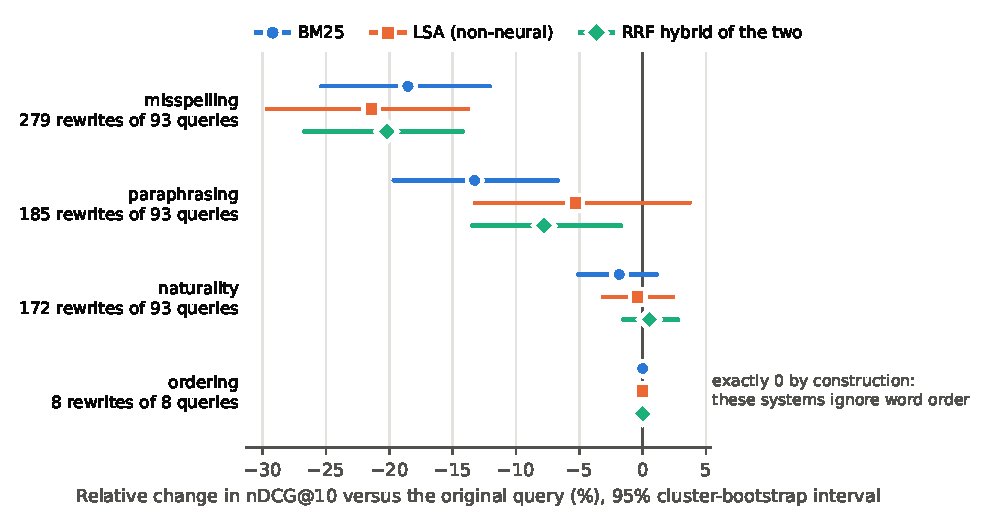
\includegraphics[width=1\textwidth,height=\textheight]{figures/fig1_ndcg_change.pdf}
\caption{Figure 1. Relative change in nDCG@10 per variation category and
system, with 95\% cluster-bootstrap intervals (data: Table 3). Ordering
is exactly zero because all three systems ignore word order, and rests
on only 8 rewrites.}
\end{figure}

\emph{Misspelling.} nDCG@10 changed by −18.5\% (95\% CI −25.4\% to
−12.1\%) for BM25, −21.4\% (95\% CI −29.7\% to −13.8\%) for LSA and
−20.2\% (95\% CI −26.7\% to −14.2\%) for the hybrid. All three
Holm-adjusted p-values are below 0.001 (the permutation test cannot
return less than about \(5 \times 10^{-6}\) with 200,000 flips). The
losses are of similar size for the three systems and the intervals
overlap heavily.

\emph{Paraphrasing.} BM25 changed by −13.3\% (95\% CI −19.7\% to −6.7\%)
(Holm p = 0.004). For LSA the change was −5.3\% (95\% CI −13.2\% to
3.7\%) (Holm p = 1.00), so no reliable change was detected. For the
hybrid it was −7.8\% (95\% CI −13.5\% to −1.7\%): the interval excludes
zero and the uncorrected permutation p-value is 0.017, but after Holm
correction it is 0.133, which does not meet the pre-specified criterion.
Section 4.4 shows that the category average hides a large difference
between its two generators.

\emph{Naturality.} Natural-language questions and stop-word removal
changed nDCG@10 by −1.9\% (BM25), −0.4\% (LSA) and 0.5\% (hybrid); all
intervals cover zero and no reliable change was detected. The point
estimates are below 2\% in absolute value.

\emph{Ordering.} The change is exactly zero for every system, which is
guaranteed by construction because BM25, LSA and their fusion are
bag-of-words systems. The category has only 8 rewrites. This row is a
check that the pipeline is order-invariant, not evidence about word
order.

\emph{Secondary measures.} Recall@100 for misspellings changed by
−10.6\% (BM25), −12.0\% (LSA) and −9.6\% (hybrid), and for paraphrasing
by −7.1\%, −5.5\% and −5.6\%; all six intervals exclude zero
(uncorrected, descriptive). Paraphrasing therefore reduced deep recall
for every system even where the nDCG@10 change for LSA was inconclusive.
MRR@10 intervals for paraphrasing cover zero for all three systems (BM25
−8.0\% (95\% CI −16.1\% to 1.0\%)).

\emph{Level versus change.} BM25 has the highest nDCG@10 after rewriting
in each of misspelling, paraphrasing and naturality (Table 3), followed
by the hybrid and then LSA, simply because it starts highest. A system
can lose less in relative terms and still be worse in absolute terms.

\hypertarget{ranking-stability-and-its-relation-to-effectiveness}{%
\subsection{Ranking stability and its relation to
effectiveness}\label{ranking-stability-and-its-relation-to-effectiveness}}

Table 4 reports how much the top of the ranking moves.

\begin{longtable}[]{@{}
  >{\raggedright\arraybackslash}p{(\columnwidth - 6\tabcolsep) * \real{0.1688}}
  >{\raggedright\arraybackslash}p{(\columnwidth - 6\tabcolsep) * \real{0.1818}}
  >{\raggedleft\arraybackslash}p{(\columnwidth - 6\tabcolsep) * \real{0.3247}}
  >{\raggedleft\arraybackslash}p{(\columnwidth - 6\tabcolsep) * \real{0.3247}}@{}}
\caption{Table 4. Ranking stability: agreement between the ranking for
the original query and the ranking for its rewrite, from the same system
(1 = identical top 10 / identical ranking; mean over queries,
cluster-bootstrap interval).}\tabularnewline
\toprule\noalign{}
\begin{minipage}[b]{\linewidth}\raggedright
System
\end{minipage} & \begin{minipage}[b]{\linewidth}\raggedright
Category
\end{minipage} & \begin{minipage}[b]{\linewidth}\raggedleft
Overlap@10 {[}95\% CI{]}
\end{minipage} & \begin{minipage}[b]{\linewidth}\raggedleft
RBO, \(p\) = 0.9 {[}95\% CI{]}
\end{minipage} \\
\midrule\noalign{}
\endfirsthead
\toprule\noalign{}
\begin{minipage}[b]{\linewidth}\raggedright
System
\end{minipage} & \begin{minipage}[b]{\linewidth}\raggedright
Category
\end{minipage} & \begin{minipage}[b]{\linewidth}\raggedleft
Overlap@10 {[}95\% CI{]}
\end{minipage} & \begin{minipage}[b]{\linewidth}\raggedleft
RBO, \(p\) = 0.9 {[}95\% CI{]}
\end{minipage} \\
\midrule\noalign{}
\endhead
\bottomrule\noalign{}
\endlastfoot
BM25 & misspelling & 0.66 {[}0.62, 0.69{]} & 0.65 {[}0.62, 0.69{]} \\
BM25 & paraphrasing & 0.55 {[}0.52, 0.59{]} & 0.53 {[}0.49, 0.57{]} \\
BM25 & naturality & 0.87 {[}0.84, 0.90{]} & 0.87 {[}0.84, 0.90{]} \\
BM25 & ordering & 1.00 {[}1.00, 1.00{]} & 1.00 {[}1.00, 1.00{]} \\
LSA & misspelling & 0.69 {[}0.65, 0.72{]} & 0.66 {[}0.63, 0.70{]} \\
LSA & paraphrasing & 0.61 {[}0.57, 0.65{]} & 0.59 {[}0.55, 0.63{]} \\
LSA & naturality & 0.91 {[}0.89, 0.94{]} & 0.91 {[}0.88, 0.93{]} \\
LSA & ordering & 1.00 {[}1.00, 1.00{]} & 1.00 {[}1.00, 1.00{]} \\
RRF hybrid & misspelling & 0.67 {[}0.63, 0.71{]} & 0.64 {[}0.60,
0.68{]} \\
RRF hybrid & paraphrasing & 0.60 {[}0.56, 0.63{]} & 0.56 {[}0.52,
0.59{]} \\
RRF hybrid & naturality & 0.90 {[}0.88, 0.93{]} & 0.89 {[}0.86,
0.92{]} \\
RRF hybrid & ordering & 1.00 {[}1.00, 1.00{]} & 1.00 {[}1.00, 1.00{]} \\
\end{longtable}

Misspelling changes the top ten less than paraphrasing does: overlap@10
is 0.66, 0.69 and 0.67 for BM25, LSA and hybrid, against 0.55, 0.61 and
0.60. Yet paraphrasing cost less nDCG@10 than misspelling for every
system (Table 3). Across categories, then, ranking stability is not a
proxy for harm: a rewrite can reshuffle the top ten into other, equally
relevant documents. Across individual (query, rewrite) pairs within a
system, however, lower RBO goes with a larger absolute nDCG@10 change:
Spearman correlation −0.67 {[}−0.74, −0.59{]} for BM25, −0.60 {[}−0.66,
−0.53{]} for LSA and −0.67 {[}−0.74, −0.60{]} for the hybrid (644 pairs;
cluster-bootstrap intervals). Part of this association is mechanical,
because a ranking that changes more has more room to change its score;
the pilot cannot separate that from a substantive link.

\hypertarget{generators-within-categories}{%
\subsection{Generators within
categories}\label{generators-within-categories}}

\begin{longtable}[]{@{}
  >{\raggedright\arraybackslash}p{(\columnwidth - 10\tabcolsep) * \real{0.1081}}
  >{\raggedright\arraybackslash}p{(\columnwidth - 10\tabcolsep) * \real{0.1892}}
  >{\raggedleft\arraybackslash}p{(\columnwidth - 10\tabcolsep) * \real{0.0811}}
  >{\raggedleft\arraybackslash}p{(\columnwidth - 10\tabcolsep) * \real{0.2072}}
  >{\raggedleft\arraybackslash}p{(\columnwidth - 10\tabcolsep) * \real{0.2072}}
  >{\raggedleft\arraybackslash}p{(\columnwidth - 10\tabcolsep) * \real{0.2072}}@{}}
\caption{Table 5. Relative change in nDCG@10 (\%) by generator, with
95\% cluster-bootstrap intervals. Descriptive only; these 24 cells are
not part of the multiplicity-corrected family.}\tabularnewline
\toprule\noalign{}
\begin{minipage}[b]{\linewidth}\raggedright
Category
\end{minipage} & \begin{minipage}[b]{\linewidth}\raggedright
Generator
\end{minipage} & \begin{minipage}[b]{\linewidth}\raggedleft
Rewrites
\end{minipage} & \begin{minipage}[b]{\linewidth}\raggedleft
BM25
\end{minipage} & \begin{minipage}[b]{\linewidth}\raggedleft
LSA
\end{minipage} & \begin{minipage}[b]{\linewidth}\raggedleft
RRF hybrid
\end{minipage} \\
\midrule\noalign{}
\endfirsthead
\toprule\noalign{}
\begin{minipage}[b]{\linewidth}\raggedright
Category
\end{minipage} & \begin{minipage}[b]{\linewidth}\raggedright
Generator
\end{minipage} & \begin{minipage}[b]{\linewidth}\raggedleft
Rewrites
\end{minipage} & \begin{minipage}[b]{\linewidth}\raggedleft
BM25
\end{minipage} & \begin{minipage}[b]{\linewidth}\raggedleft
LSA
\end{minipage} & \begin{minipage}[b]{\linewidth}\raggedleft
RRF hybrid
\end{minipage} \\
\midrule\noalign{}
\endhead
\bottomrule\noalign{}
\endlastfoot
misspelling & \texttt{NeighbCharSwap} & 93 & −18.1 {[}−26.4, −9.8{]} &
−21.3 {[}−31.2, −11.7{]} & −20.0 {[}−28.4, −12.0{]} \\
misspelling & \texttt{RandomCharSub} & 93 & −15.5 {[}−23.7, −7.7{]} &
−17.9 {[}−27.7, −8.7{]} & −18.1 {[}−25.7, −10.8{]} \\
misspelling & \texttt{QWERTYCharSub} & 93 & −22.0 {[}−29.8, −14.3{]} &
−25.0 {[}−36.0, −14.2{]} & −22.5 {[}−31.2, −14.4{]} \\
paraphrasing & \texttt{LLM\_Paraphrase} & 93 & −8.6 {[}−15.7, −1.1{]} &
0.9 {[}−7.9, 10.5{]} & −0.9 {[}−7.9, 6.6{]} \\
paraphrasing & \texttt{LLM\_SynonymSwap} & 92 & −18.5 {[}−27.6, −9.5{]}
& −12.1 {[}−23.5, −0.1{]} & −15.2 {[}−23.7, −6.6{]} \\
naturality & \texttt{LLM\_NaturalQuestion} & 92 & −1.7 {[}−6.6, 3.2{]} &
−1.1 {[}−5.2, 3.1{]} & 1.1 {[}−2.4, 4.8{]} \\
naturality & \texttt{RemoveStopWords} & 80 & 0.1 {[}−1.4, 1.9{]} & 0.0
{[}−3.1, 3.1{]} & −0.1 {[}−2.1, 2.3{]} \\
ordering & \texttt{RandomOrderSwap} & 8 & 0.0 {[}0.0, 0.0{]} & 0.0
{[}0.0, 0.0{]} & 0.0 {[}0.0, 0.0{]} \\
\end{longtable}

Within misspelling all three generators lower nDCG@10 for every system
(all intervals below zero), and the QWERTY-neighbour substitution is the
most damaging for all three. Within paraphrasing the two generators
differ greatly: the synonym swap changes BM25 by −18.5\%, about as much
as a typo, whereas the structural paraphrase changes it by −8.6\%; for
LSA the structural paraphrase is indistinguishable from zero (0.9\%
(95\% CI −7.9\% to 10.5\%)) and the synonym swap costs −12.1\%. The
synonym swap is the most damaging non-typo generator for every system.
The category average of Table 3 is therefore an average over two
different phenomena, and its size depends on how many rewrites each
generator contributes. A reading consistent with these data, but not
tested here, is that replacing query words by words that do not occur in
the relevant documents hurts every system that matches words, while a
latent space softens part of that loss. Within naturality both
generators are close to zero.

\hypertarget{the-hybrid-compared-with-its-components-exploratory}{%
\subsection{The hybrid compared with its components
(exploratory)}\label{the-hybrid-compared-with-its-components-exploratory}}

\begin{longtable}[]{@{}
  >{\raggedright\arraybackslash}p{(\columnwidth - 4\tabcolsep) * \real{0.1842}}
  >{\raggedleft\arraybackslash}p{(\columnwidth - 4\tabcolsep) * \real{0.4079}}
  >{\raggedleft\arraybackslash}p{(\columnwidth - 4\tabcolsep) * \real{0.4079}}@{}}
\caption{Table 6. Exploratory comparison of the hybrid with its
components: mean per-query difference in the \emph{absolute} nDCG@10
change (hybrid minus component) with a 95\% cluster-bootstrap interval.
Positive means the hybrid lost less (or gained more) than the component.
No test, no multiplicity correction.}\tabularnewline
\toprule\noalign{}
\begin{minipage}[b]{\linewidth}\raggedright
Category
\end{minipage} & \begin{minipage}[b]{\linewidth}\raggedleft
RRF hybrid minus BM25
\end{minipage} & \begin{minipage}[b]{\linewidth}\raggedleft
RRF hybrid minus LSA
\end{minipage} \\
\midrule\noalign{}
\endfirsthead
\toprule\noalign{}
\begin{minipage}[b]{\linewidth}\raggedright
Category
\end{minipage} & \begin{minipage}[b]{\linewidth}\raggedleft
RRF hybrid minus BM25
\end{minipage} & \begin{minipage}[b]{\linewidth}\raggedleft
RRF hybrid minus LSA
\end{minipage} \\
\midrule\noalign{}
\endhead
\bottomrule\noalign{}
\endlastfoot
misspelling & +0.003 {[}−0.014, +0.021{]} & −0.017 {[}−0.033,
−0.001{]} \\
paraphrasing & +0.028 {[}+0.005, +0.051{]} & −0.015 {[}−0.035,
+0.005{]} \\
naturality & +0.010 {[}−0.002, +0.024{]} & +0.003 {[}−0.004,
+0.011{]} \\
ordering & 0.000 {[}0.000, 0.000{]} & 0.000 {[}0.000, 0.000{]} \\
\end{longtable}

In relative terms the hybrid's change lies between those of BM25 and LSA
for misspelling and for paraphrasing (Table 3). In the pre-specified,
exploratory comparison of absolute changes (hybrid minus component;
positive means the hybrid lost less), the difference to BM25 under
paraphrasing was +0.028 {[}+0.005, +0.051{]}, an interval above zero,
and there is no clear difference to BM25 under misspelling (+0.003
{[}−0.014, +0.021{]}). Against LSA under misspelling the difference was
−0.017 {[}−0.033, −0.001{]}, so the hybrid lost more in absolute terms;
this comparison is confounded by level, since LSA starts lower and has
less to lose. These contrasts must not be read as ``the hybrid is more
robust than BM25'': after paraphrasing the hybrid's nDCG@10 (0.352) is
still below BM25's (0.374), and the hybrid is also below BM25 on the
original queries.

\hypertarget{sensitivity-to-the-validity-rule}{%
\subsection{Sensitivity to the validity
rule}\label{sensitivity-to-the-validity-rule}}

The whole analysis was repeated with the reviewer's labels alone,
without the stricter recheck (47 word-order swaps instead of 8). Every
estimate for misspelling and paraphrasing is identical to the main run,
because the recheck touches only word-order swaps and stop-word removal.
The naturality change moves from −1.9\% to −1.8\% (BM25), from −0.4\% to
−0.5\% (LSA) and from 0.5\% to 0.5\% (hybrid), ordering stays exactly
zero, no Holm decision changes, and the Spearman correlations change
from −0.67, −0.60, −0.67 to −0.70, −0.63, −0.70. The conclusions do not
depend on this choice. They do depend on the more basic assumption that
the kept rewrites preserve meaning, which this sensitivity analysis
cannot test.

\hypertarget{a-diagnostic-on-the-typo-rewrites}{%
\subsection{A diagnostic on the typo
rewrites}\label{a-diagnostic-on-the-typo-rewrites}}

0 of the 279 typo rewrites turned the edited word into another word that
occurs in the collection, and the reviewer judged all 30 calibration
typos equivalent. For models that match whole words, an edited query
word then most likely stops matching altogether, so a typo behaves like
deleting the term. This explanation fits the size of the typo losses but
was not tested here; the direct test (rewrites that delete the same
word) is an obvious next experiment. It need not carry over to
retrievers with sub-word tokenisation, which prior work reports are
affected by typos too \citep{zhuang2021, sidiropoulos2022}.

\hypertarget{discussion}{%
\section{Discussion}\label{discussion}}

The most robust finding of the pilot is the cost of misspellings: about
a fifth of nDCG@10 for all three whole-word systems, with intervals far
from zero, similar across systems and of the same order for the three
typo generators (Table 5). Losses of this size are in the range that
\citet{penha2022} report for their pipelines (read through a summariser;
see Appendix A), but the collections, systems, generators and measures
differ, so the numbers are not comparable and no agreement or
disagreement is claimed.

The paraphrasing result is more qualified than a first glance at Table 3
suggests. The reliable loss for BM25 comes largely from the synonym
swap; the structural paraphrase costs BM25 less and LSA nothing
detectable. Whether a category average is informative therefore depends
on its generators, and a study that reports only category averages can
mislead. This is a caution about reporting, not a new effect.
\citet{li2026} report that LLM-based dense retrievers, although more
robust to typos than encoder-only baselines, remain vulnerable to
synonym substitution; here the synonym swap is also among the most
damaging non-typo variations, but the systems and measures differ and
that source was read at abstract level only, so this is a similarity of
direction and nothing more.

Stability and harm come apart across categories (Section 4.3). A
practitioner who monitors only how much the top ten moves would rank
paraphrasing as the more disruptive variation, while the effectiveness
loss is larger for misspelling. Both quantities are worth reporting, and
neither replaces the other. The within-system correlation also shows
that, rewrite by rewrite, instability is informative about harm in this
pilot.

For the hybrid, the pilot gives a modest, hedged picture. Its relative
losses lie between those of its components, and under paraphrasing it
lost less than BM25 in absolute nDCG@10 (exploratory), but its level on
the original queries is lower than BM25's. Because both components are
whole-word models that share a vocabulary and an analyzer, the hybrid
cannot show the complementarity a neural retriever might add. The
question that motivated the design, whether a fused lexical-neural first
stage is more robust than either component, remains open.

If the typo effect held on other collections, the first thing to check
for lexical and LSA-style first stages would be query normalisation or
typo-tolerant matching. The pilot cannot say whether it holds elsewhere.

\hypertarget{limitations}{%
\section{Limitations}\label{limitations}}

\begin{itemize}
\tightlist
\item
  \textbf{One small, old collection} (93 queries, abstracts from the
  1960s), whose provenance and licence are unclear and whose Glasgow
  page carries a caution. Nothing here generalises to other domains or
  to modern query logs.
\item
  \textbf{No neural retriever.} LSA is non-neural; the hybrid combines
  two whole-word systems. The pilot says nothing about neural dense
  retrievers or about neural-plus-lexical hybrids.
\item
  \textbf{No human verification of any rewrite.} Validity rests on
  construction (typos), one LLM reviewer from the generator's model
  family, and a stricter recheck by the same assistant that wrote the
  code. No inter-annotator agreement exists. If the kept rewrites are
  not all meaning-preserving, the effects are overstated.
\item
  \textbf{Rewrites written by the same AI system that wrote the code and
  the analysis.} There was no separate prompt or seed, so the
  LLM-written rewrites cannot be regenerated.
\item
  \textbf{Word order is untestable here}: the three systems ignore it by
  construction, and only 8 rewrites remain.
\item
  \textbf{Unequal contributions.} Rewrites per query differ across
  generators and categories; the primary analysis averages within query
  to keep queries independent, but the category averages still depend on
  the generator mix (Section 4.4).
\item
  \textbf{Multiplicity and power.} Twelve primary tests, 93 queries,
  wide intervals. The hybrid's paraphrasing result is neither confirmed
  nor refuted. Generator-level, secondary-measure and hybrid-comparison
  results are descriptive.
\item
  \textbf{Single seed and untuned own BM25.} One LSA seed; BM25
  parameters are defaults, not tuned, and the implementation
  approximates but does not equal Elasticsearch's analyzer.
\item
  \textbf{The explanation that typos act like term deletion is a
  hypothesis.}
\item
  \textbf{The literature search was not systematic} and several sources
  were read only through abstracts or a page summariser (Appendix A);
  the gap statement may be wrong.
\item
  \textbf{AI-authored.} Code, rewrites, review, analysis and text came
  from an AI system (Section 8). The automated checks reduce but do not
  remove the chance of error.
\end{itemize}

\hypertarget{reproducibility-and-availability}{%
\section{Reproducibility and
availability}\label{reproducibility-and-availability}}

The repository contains the package (\texttt{src/qvr}), the scripts, the
85 tests, the rewrite files with their review records, the saved
rankings of every system for every query and rewrite, the per-query
tables, the analysis plan and this manuscript's builder. The run took
about 10.02 seconds on one CPU in the sandbox (Python 3.13.16, numpy
2.5.4, scipy 1.18.1, pandas 3.0.5, scikit-learn 1.9.1, snowballstemmer
3.1.1). The commands are \texttt{python\ scripts/fetch\_vaswani.py},
\texttt{python\ scripts/run\_experiment.py\ ...},
\texttt{python\ scripts/analyze.py\ ...},
\texttt{python\ scripts/build\_paper.py} and
\texttt{python\ scripts/verify\_results.py}; the README lists them in
full. The BM25, LSA and RRF code is deterministic given the seeds; a
re-run in a fresh environment with other library versions gave the same
per-query tables and the same document order in every ranked list, with
stored LSA scores differing only in the seventh decimal
(\texttt{results/reproduction\_check.md}). The repository address is
{[}REPOSITORY URL: to be confirmed by the author{]}. The Vaswani files
are not included; \texttt{fetch\_vaswani.py} retrieves and checks them.

\hypertarget{ai-assistance-authorship-and-responsibility}{%
\section{AI assistance, authorship and
responsibility}\label{ai-assistance-authorship-and-responsibility}}

\emph{{[}HUMAN AUTHOR TO COMPLETE AND CONFIRM. This section was drafted
by the AI system and does not replace the authors' own statement.{]}}

The software, the tests, the 279 LLM-written query rewrites, the
experiment runs, the analysis plan, the checks and this text were
produced in one working session with Claude (Anthropic); the session was
configured as Claude Sonnet 5.5, and the serving model cannot be
verified from inside the session. Code produced 455 further rewrite
candidates. A smaller Claude model setting acted as the blind reviewer
of rewrite validity. The AI system cannot be an author and cannot take
responsibility for the content; arXiv's policy states that generative AI
tools should not be listed as authors, that authors take full
responsibility for all contents irrespective of how they were generated,
and that significant use of such tools should be reported
\citep{arxiv_ai_policy}. Before this work is submitted anywhere, the
human author(s) must at least:

\begin{itemize}
\tightlist
\item
  read the whole manuscript, the code and the data, and decide what is
  claimed;
\item
  re-run \texttt{pytest} and \texttt{python\ scripts/verify\_results.py}
  and confirm the numbers;
\item
  check every citation against the cited paper, in particular the claims
  that rest on abstracts or on a page summariser (Appendix A);
\item
  decide whether a pilot of this scope should be submitted at all, or
  first extended (Appendix B);
\item
  write their own statement of contributions and of AI use that matches
  what they actually did.
\end{itemize}

\hypertarget{conclusion}{%
\section{Conclusion}\label{conclusion}}

On one small collection, misspellings cost BM25, LSA and their RRF
hybrid about a fifth of nDCG@10 (all Holm-adjusted p-values below
0.001). Paraphrasing cost BM25 13.3\% but did not reliably change LSA
or, after correction, the hybrid. Natural-question and stop-word
rewrites changed little, and word order cannot matter for these systems.
Ranking stability and effectiveness loss are linked within a system but
not comparable across categories. The pilot's value is a verified,
reproducible pipeline and a set of effect sizes; its weaknesses are the
absence of neural retrievers, of other collections and of any human
validation of the rewrites. The research question that motivated it, how
a fused lexical-neural first stage behaves under query variation, is not
answered.

\hypertarget{references}{%
\section*{References}\label{references}}
\addcontentsline{toc}{section}{References}

\bibliography{references}

\hypertarget{appendix-a-literature-search-record}{%
\section*{Appendix A: Literature search
record}\label{appendix-a-literature-search-record}}
\addcontentsline{toc}{section}{Appendix A: Literature search record}

\textbf{What was done.} A general web search engine (standard and
extended modes; results are titles and links only) and direct reads of
arXiv listings, the ACL Anthology, Crossref records and publisher pages.
DBLP could not be used (blocked for automated access). Google Scholar,
the ACM Digital Library and Semantic Scholar search were not used. No
systematic-review protocol was followed. Inclusion rule applied by title
and abstract: the item studies the robustness of retrieval (first stage,
dense or re-ranking) to the wording of queries (typos, paraphrases,
variants) or the consistency of rankings across variants. Items about
retrieval-augmented generation only, generative retrieval only, or
adversarial corpus attacks were noted but not used. The record of
searches made at the very start of the work was lost when the working
session's context was compacted; the searches below are those that could
be recovered from session logs or were made afterwards. A human author
should repeat and log the search before relying on the gap statement.

\begin{longtable}[]{@{}
  >{\raggedright\arraybackslash}p{(\columnwidth - 6\tabcolsep) * \real{0.0615}}
  >{\raggedright\arraybackslash}p{(\columnwidth - 6\tabcolsep) * \real{0.2000}}
  >{\raggedright\arraybackslash}p{(\columnwidth - 6\tabcolsep) * \real{0.5692}}
  >{\raggedright\arraybackslash}p{(\columnwidth - 6\tabcolsep) * \real{0.1692}}@{}}
\caption{Table 7. Searches that could be recovered or were made
afterwards (dates are those of the run; the earlier ones are from the
sub-agent's log, in UTC).}\tabularnewline
\toprule\noalign{}
\begin{minipage}[b]{\linewidth}\raggedright
\#
\end{minipage} & \begin{minipage}[b]{\linewidth}\raggedright
Date
\end{minipage} & \begin{minipage}[b]{\linewidth}\raggedright
Query
\end{minipage} & \begin{minipage}[b]{\linewidth}\raggedright
Mode
\end{minipage} \\
\midrule\noalign{}
\endfirsthead
\toprule\noalign{}
\begin{minipage}[b]{\linewidth}\raggedright
\#
\end{minipage} & \begin{minipage}[b]{\linewidth}\raggedright
Date
\end{minipage} & \begin{minipage}[b]{\linewidth}\raggedright
Query
\end{minipage} & \begin{minipage}[b]{\linewidth}\raggedright
Mode
\end{minipage} \\
\midrule\noalign{}
\endhead
\bottomrule\noalign{}
\endlastfoot
1 & 2026-10-17 & query variation robustness first-stage retrieval BM25
dense hybrid & standard \\
2 & 2026-10-17 & typos robustness hybrid retrieval BM25 dense fusion &
standard \\
3 & 2026-10-17 & paraphrase robustness BEIR dense retrievers query
reformulation sensitivity & standard \\
4 & 2026-10-17 & ranking stability query variants rank-biased overlap
neural retrieval & standard \\
5 & 2026-10-17 & LLM-generated query variants meaning-preserving
validation retrieval robustness benchmark & extended \\
6 & 2026-10-17 & query variations robustness retrieval 2026 arXiv &
extended \\
7 & 2026-10-17 & ``query variation'' retrieval robustness & standard \\
8 & 2026-10-17 & typos dense retrieval & standard \\
9 & 2026-10-17 & paraphrase robustness retrieval & standard \\
10 & 2026-10-17 & hybrid retrieval robustness & standard \\
11 & 2026-10-22 & hybrid retrieval BM25 dense reciprocal rank fusion
robustness to query typos and paraphrases evaluation & standard \\
12 & 2026-10-22 & query variation generators misspelling ordering
naturality paraphrasing retrieval robustness first-stage retrievers &
standard \\
13 & 2026-10-22 & lexical versus dense retrieval typo robustness BM25
misspelled queries comparison study & standard \\
14 & 2026-10-22 & ranking stability across query variants rank-biased
overlap relationship with effectiveness change & standard \\
15 & 2026-10-22 & LLM-generated query variants validity human judgment
same information need retrieval evaluation & standard \\
\end{longtable}

Searches 11 and 12 again returned the papers already known
\citep{penha2022, li2026} and no study of a fused lexical-semantic first
stage under query variations; search 10 returned nothing on that topic
either. Searches 13 to 15 returned the typo-robustness, consistency and
LLM-query-variant papers already cited, plus the items listed below as
seen by title only. The results are only titles, so ``returned nothing''
means that no title suggested it.

\textbf{How each cited source was read.} ``Record'' means a
bibliographic record only (title, authors, venue, pages). ``Abstract''
means the abstract or listing page. ``Summariser'' means the full text
through a page-summarising tool, whose output can be wrong and must be
checked against the PDF.

\begin{longtable}[]{@{}
  >{\raggedright\arraybackslash}p{(\columnwidth - 4\tabcolsep) * \real{0.3295}}
  >{\raggedright\arraybackslash}p{(\columnwidth - 4\tabcolsep) * \real{0.3182}}
  >{\raggedright\arraybackslash}p{(\columnwidth - 4\tabcolsep) * \real{0.3523}}@{}}
\caption{Table 8. Reading level of each cited source.}\tabularnewline
\toprule\noalign{}
\begin{minipage}[b]{\linewidth}\raggedright
Source
\end{minipage} & \begin{minipage}[b]{\linewidth}\raggedright
Read
\end{minipage} & \begin{minipage}[b]{\linewidth}\raggedright
Used for
\end{minipage} \\
\midrule\noalign{}
\endfirsthead
\toprule\noalign{}
\begin{minipage}[b]{\linewidth}\raggedright
Source
\end{minipage} & \begin{minipage}[b]{\linewidth}\raggedright
Read
\end{minipage} & \begin{minipage}[b]{\linewidth}\raggedright
Used for
\end{minipage} \\
\midrule\noalign{}
\endhead
\bottomrule\noalign{}
\endlastfoot
\citet{penha2022} & abstract page, Crossref record, full text through a
summariser, authors' repository README & taxonomy, generators, datasets
and systems used, size of the average loss, validation by the authors \\
\citet{hagen2024} & ACL Anthology page and abstract, Crossref record,
full text through a summariser & scope (re-rankers, newer models),
statement that the re-ranking stage is evaluated \\
\citet{li2026} & arXiv abstract page & robustness of LLM-based dense
retrievers, typo and synonym findings \\
\citet{percin2025} & arXiv abstract page & RAG retrievers degrade under
minor variations \\
\citet{campese2025} & arXiv page, abstract summary only (submission date
not shown) & consistency loss for equivalent queries \\
\citet{sidiropoulos2022}, \citet{sidiropoulos2024} & Crossref record;
arXiv abstract page & typo robustness of dense retrievers \\
\citet{zhuang2021}, \citet{tasawong2023} & ACL Anthology pages & typo
robustness of neural retrieval \\
\citet{zhuang2022} & Crossref record & typo robustness of dense
retrievers \\
\citet{alaofi2023} & Crossref record only & LLM-generated query
variants \\
\citet{bailey2016}, \citet{bailey2017}, \citet{moffat2015} &
bibliographic records & query variability and consistency \\
\citet{thakur2021} & arXiv listing (version 4); venue taken from a
proceedings link in search results, not opened & BEIR, planned
follow-up \\
\citet{cormack2009}, \citet{webber2010}, \citet{jarvelin2002},
\citet{smucker2007}, \citet{vangysel2018} & bibliographic records
(Crossref, Webis anthology) & methods used; implementations checked
against independent software \\
\citet{robertson2009}, \citet{deerwester1990}, \citet{porter1980} &
publisher or index pages & methods used \\
\citet{holm1979} & GESIS knowledge-graph record (title, journal, volume,
issue, pages; the author is inferred from the record identifier) &
multiplicity correction \\
\citet{irdatasets_vaswani}, \citet{glasgow_npl} & the web pages &
collection description \\
\citet{arxiv_ai_policy} & the arXiv blog post & AI-use and authorship
policy \\
\end{longtable}

\textbf{Items seen in search results by title only, not read and not
relied on:} on robustness of generative retrieval (arXiv 2306.12756;
arXiv 2412.18768), adaptive RAG robustness to query variations (arXiv
2604.10745), a study of LLM-based retrievers on BRIGHT including query
perturbations (arXiv 2604.03676), query rewriting for retrieval (arXiv
2407.12529, 2603.13301), zero-shot hybrid retrieval models (ECIR 2022),
demographically inspired LLM query variants (arXiv 2508.17644), LLM
query simulation and answer-side intrusion (arXiv 2608.25245), and
rank-similarity measures based on maximised effectiveness difference
(arXiv 1408.3587).

\textbf{Claims that depend on a summariser's reading of full text and
must be checked by the human author:} the roughly 20\% average loss and
the datasets and systems used by \citet{penha2022}; that neither
\citet{penha2022} nor \citet{hagen2024} evaluates a fused
lexical-semantic first stage; that \citet{hagen2024} evaluate the
re-ranking stage.

\hypertarget{appendix-b-what-a-stronger-study-needs}{%
\section*{Appendix B: What a stronger study
needs}\label{appendix-b-what-a-stronger-study-needs}}
\addcontentsline{toc}{section}{Appendix B: What a stronger study needs}

\begin{enumerate}
\def\labelenumi{\arabic{enumi}.}
\tightlist
\item
  At least two neural dense retrievers, chosen and documented before
  running, with their hybrids with BM25, on at least three BEIR domains
  (instructions: \texttt{docs/RUN\_BEIR\_LOCALLY.md}).
\item
  Human validation of the rewrites by at least two annotators, with
  agreement reported (the blind audit sheet and tool are in the
  repository), and logged prompts and decoding settings for the
  LLM-written rewrites.
\item
  A term-deletion control for the typo rewrites and a generator-level
  pre-specification for paraphrasing.
\item
  A systematic literature search with a written protocol, a log of
  queries and databases, and a full-text reading of the closest papers.
\item
  A pre-registered analysis plan with an external timestamp.
\end{enumerate}

\end{document}
